
\chapter{Week 12}

\section{Monday}\index{Monday_lecture}
We will introduce three continuous time stochastic processes, the first two of which have \emph{independent increments}.
They naturally arise in many applications, but their sample paths are quite different from the discrete time case, since the sample paths of continuous time processes are functions on $\mathbb{R}_+$.
The two extremes of these sample paths are:
\begin{itemize}
\item
Only changes discontinuously, i.e., piecewise step function;
\item
Only changes continuously, i.e., continuous function of time.
\end{itemize}
A typical example of i) is a Possion process, while the example of ii) is a Brownian motion.

In general, a real-valued process with independent increments is called a Levy process.
In this week, we will discuss another process, the continuous time Markov chain,
It relaxes the independent increment condition, and it is a natural extension of discrete time Markov chain.
The Possion process is a special case of CTMC. We will study this process first, and it will motivate us to study a general continuous time Markoc chain, or further continuous time Markov process.

\subsection{Poisson Process}
\begin{definition}[Simple Counting Process]
A non-negative integer-valued process $N(\cdot)\equiv\{N(t):~t\ge0\}$ is called a simple counting process,
if $N(0)=0$, and $N(t)$ is piecewise constant in $t\ge0$, and $\Delta N(t)\equiv N(t)-N(t-)$ is either $0$ or $1$ for all $t\ge0$.
\end{definition}

\begin{definition}[Poisson Process]
If a simple counting process $N(\cdot)$ adapted to $\mathbb{F}$ satisfies
\begin{enumerate}
\item
For all $s,t>0$, $N(s+t)-N(s)$ is independent of $\mathcal{F}_s$;
\item
For any $s,t>0$, $N(t)\overset{d}{\sim}N(s+t)-N(s)$;
\item
$\lambda\equiv \mathbb{E}[N(1)]<\infty$ and $\lambda>0$,
\end{enumerate}
then $N(\cdot)$ is called a time-homogeneous Poisson process with intensity $\lambda$.
\end{definition}

\begin{theorem}[Martingale Characterization of Poisson Process]
Let $N(\cdot)$ be a simple counting process and define $M(\cdot)$ by
\[
M(t)=N(t)-\lambda t,\quad t\ge0,
\]
then $N(\cdot)$ is a Poisson process with intensity $\lambda$ if and only if $M(\cdot)$ is a martingale.
\end{theorem}
We will make use of the following fact for showing this theorem:
\begin{quotation}
Suppose that $f$ is a right-continuous function from $\mathbb{R}_+$ to $\mathbb{R}$.
Then for $\forall s,t\ge0$, $f(s+t)=f(s)+f(t)$ holds if and only if $f(t)=f(1)t$.
\end{quotation}
\begin{proof}
Assume that $M(\cdot)$ is a Poisson process, then $\mathbb{E}[N(s+t)]=\mathbb{E}[N(s)]+\mathbb{E}[N(t)]$, which implies $\mathbb{E}[N(t)]=\lambda t$.
Furthremore, for $0\le s<t$,
\begin{align*}
\mathbb{E}[M(t)\mid\mathcal{F}_s]&=\mathbb{E}[N(t)\mid\mathcal{F}_s]-\lambda t\\
&=N(s)+\mathbb{E}[N(t)-N(s)\mid\mathcal{F}_s]-\lambda t\\
&=N(s)+\mathbb{E}[N(t-s)]-\lambda t=N(s)-\lambda s=M(s).
\end{align*}
Moreover, $\mathbb{E}[|M(t)|]\le 2\lambda t$, which implies $M(\cdot)$ is a martingale.

Conversely, suppose that $M(\cdot)$ is a martingale.
Then $\mathbb{E}[N(t)]=\lambda t<\infty$, so 3) for Poisson process holds.
We use the test function $e^{\theta x}, \theta<0$ to study the distribution of $N(t)$.
Denote $\Delta N(t) = N(t) - N(t-)$, then for $s<t$, 
\begin{align*}
e^{\theta N(t)} - e^{\theta N(s)}&=\sum_{\Delta N(u)>0}(e^{\theta N(u)} - e^{\theta N(u-)})1(s<u\le t)\\
&=(e^{\theta}-1)\int_s^te^{\theta N(u-)}\diff N(u)\\
&=(e^{\theta}-1)\left[\int_s^te^{\theta N(u)}\lambda\diff u
+\int_s^te^{\theta N(u-)}\diff M(u)
\right]
\end{align*}
Define $Y(t)=\int_0^te^{\theta N(u-)}\diff M(u)$ and $\sigma_n=\inf\{t\ge0:~N(t)=n\}$. 
Then we have
\[
\int_{\sigma_{n-1}}^{\sigma_n}e^{\theta N(u-)}\diff M(u) = e^{\theta(n-1)}[M(\sigma_n) - M(\sigma_{n-1})].
\]
Therefore,
\begin{align*}
\int_{0}^{t}e^{\theta N(u-)}\diff M(u)&=\sum_{n=1}^\infty
\int_{\sigma_{n-1}\land t}^{\sigma_n\land t}e^{\theta N(u-)}\diff M(u)\\
&=\sum_{n=1}^\infty
 e^{\theta(n-1)}[M(\sigma_n\land t) - M(\sigma_{n-1}\land t)],
\end{align*}
and thus
\[
\int_s^te^{\theta N(u-)}\diff M(u)=Y(t)-Y(s)=\sum_{n=1}^\infty
 e^{\theta(n-1)}[M((s\lor\sigma_n)\land t) - M((s\lor\sigma_{n-1})\land t)].
\]
It follows that
\begin{align*}
e^{\theta N(t)} - e^{\theta N(s)}&=(e^{\theta}-1)\bigg[\int_s^te^{\theta N(u)}\lambda\diff u\\&+\sum_{n=1}^\infty
 e^{\theta(n-1)}[M((s\lor\sigma_n)\land t) - M((s\lor\sigma_{n-1})\land t)]
\bigg]
\end{align*}
By optional sampling theorem, $\mathbb{E}[M((s\lor\sigma_n)\land t)\mid\mathcal{F}_s] = \mathbb{E}[M((s\lor\sigma_{n-1})\land t)\mid\mathcal{F}_s]=M(s)$, and thus 
\begin{align*}
\mathbb{E}[e^{\theta N(t)} - e^{\theta N(s)}\mid\mathcal{F}_s] =(e^{\theta}-1)\lambda\mathbb{E}\bigg[\int_s^te^{\theta N(u)}\diff u\bigg|\mathcal{F}_s\bigg]
\end{align*}
Dividing both sides by $e^{\theta N(s)}$ gives
\[
\mathbb{E}[\exp(\theta(N(t) - N(s)))\mid\mathcal{F}_s] =\lambda(e^{\theta}-1)
\int_s^t\mathbb{E}[\exp(\theta(N(u) - N(s)))\mid\mathcal{F}_s]\diff u
\]
Differentiate both sides and by initial value, 
\begin{equation}
\mathbb{E}[\exp(\theta(N(t) - N(s)))\mid\mathcal{F}_s] = e^{-\lambda(t-s)(1-e^{\theta})}=\mathbb{E}[e^{\theta N(t-s)}].
\end{equation}
This shows the property 2 for Poisson process.
From the equation above, we can also see that $N(t)-N(s)$ is independent of $\mathcal{F}_s$, so property 1 is also shown.
\end{proof}
From the proof we can see that $\mathbb{E}[e^{\theta N(t)}]=\exp(-\lambda t(1-e^{\theta}))$, which implies the following corollary:
\begin{corollary}
If $N(\cdot)$ is the Poisson process with intensity $\lambda$, then $N(t)$ has the Poisson distribution with mean $\lambda$:
\[
\mathbb{P}(N(t)=k) = \frac{1}{k!}(\lambda t)^ke^{-\lambda t}
\]
\end{corollary}
Therefore, a probability measure exists on which the Poisson process $N(\cdot)$ is uniquely defined.
The next theorem answers it in another perspective:
\begin{theorem}[Inter-Counting Time Characterization of Poisson Process]
A simple counting process $N(\cdot)$ is a Poisson process with intensity $\lambda>0$,
if and only if, for $\sigma_n=\inf\{t\ge0:~N(t)\ge n\}$ we have
\begin{itemize}
\item
$T_n=\sigma_n - \sigma_{n-1}$ are i.i.d. with $\mathbb{P}(T_n\le x) = 1-e^{-\lambda x}, x\ge0$.
\end{itemize}
\end{theorem}
\begin{proof}
\begin{itemize}
\item
Assume that $N(\cdot)$ is Poisson with intensity $\lambda$, and $X(t)=\exp(\theta N(t) + \lambda t(1-e^{\theta}))$. Then $X(\cdot)$ is a martingale.
By the optinal sampling theorem for stopping times $\sigma_n^{(k)}=\sigma_n\land k, \sigma_{n-1}^{(k)}=\sigma_{n-1}\land k$, we have
\[
\mathbb{E}\bigg[
e^{\theta N(\sigma_n^{(k)}) + \lambda\sigma_n^{(k)}(1-e^{\theta})}\bigg|\mathcal{F}_{\sigma_{n-1}^{(k)}}
\bigg]=X(\sigma_{n-1}^{(k)})=
e^{\theta N(\sigma_{n-1}^{(k)}) + \lambda\sigma_{n-1}^{(k)}(1-e^{\theta})}
\]
Taking $k\to\infty$ gives
\[
\mathbb{E}[e^{\theta + \lambda(\sigma_n - \sigma_{n-1})(1-e^{\theta})}\mid \mathcal{F}_{\sigma_{n-1}}]=1.
\]
Define $u=-\lambda(1-e^{\theta})$.
It follows that
\[
\mathbb{E}[e^{-T_nu}\mid \mathcal{F}_{\sigma_{n-1}}]=e^{-\theta}=\frac{\lambda}{\lambda + u}.
\]
\item
Conversely, assume the property holds, then we first show the following equality by induction:
\[
\mathbb{P}(N(t)\le\ell)=\mathbb{P}(\sigma_{\ell+1}>t)=\sum_{k=0}^{\ell}\frac{(\lambda t)^k}{k!}e^{-\lambda t}.
\]
This holds for $\ell=0$. Assume that it holds for a given $\ell\ge0$, then
\begin{align*}
\mathbb{P}(\sigma_{\ell+2}>t)&=\mathbb{P}(\sigma_1>t) + \mathbb{P}(\sigma_1\le t, \sigma_{\ell+2}-\sigma_1+\sigma_1>t)\\
&=e^{-\lambda t} + \int_0^t\mathbb{P}(\sigma_{\ell+2}-\sigma_1+u>t)\diff F(u)\\
&=e^{-\lambda t} + \int_0^t\mathbb{P}(\sigma_{\ell+1}+u>t)\lambda e^{-\lambda u}\diff u\\
&=\sum_{k=0}^{\ell+1}\frac{(\lambda t)^k}{k!}e^{-\lambda t}.
\end{align*}
It follows that $\frac{\diff}{\diff u}\mathbb{P}(\sigma_n\le u)=\frac{\lambda^nu^{n-1}}{(n-1)!}e^{-\lambda u}$. Hence, 
\begin{align*}
\mathbb{P}&(N(s)=k, N(t)-N(s)\le \ell)\\&=
\mathbb{P}(\sigma_k\le s<\sigma_{k+1}, \sigma_{k+1}>t)
+
\mathbb{P}(\sigma_k\le s<\sigma_{k+1}, \sigma_{k+1}\le t, \sigma_{k+\ell+1}>t)\\
&=
\mathbb{P}(\sigma_k\le s, \sigma_{k+1}>t)
+
\mathbb{P}(\sigma_k\le s<\sigma_{k+1}\le t, \sigma_{k+\ell+1}-\sigma_{k+1}+\sigma_{k+1}>t)\\
&=
\int_0^s\mathbb{P}(T_k>t-u)\diff_u\mathbb{P}(\sigma_k\le u)
\\&+
\int_0^s\int_{s-u}^{t-u}\mathbb{P}(\sigma_{\ell}>t-(u+v))\diff_v\mathbb{P}(T_k\le v)\diff_u\mathbb{P}(\sigma_k\le u)\\
&=\mathbb{P}(N(s)=k)\mathbb{P}(N(t-s)\le\ell)
\end{align*}
From this equality we have 
\[
\mathbb{P}(N(s)=k, N(t)-N(s)\le \ell)=
\mathbb{P}(N(s)=k) \mathbb{P}(N(t)-N(s)\le \ell)
\]
Similarly, $\mathbb{P}(A\cap \{N(s)=k, N(t)-N(s)\le \ell\}) = \mathbb{P}(A\cap\{N(s)=k\})
\mathbb{P}(N(t)-N(s)\le\ell),\quad A\in\mathcal{F}_s
$.
As a result,
\[
\mathbb{E}[N(t)-N(s)\mid\mathcal{F}_s] = \mathbb{E}[N(t) - N(s)]=\lambda(t-s).
\]
Hence, $N(t)-\lambda t$ is a martingale, which implies $N(\cdot)$ is a Poisson process.
\end{itemize}
\end{proof}

\subsection{Brownian Motion}
A Poisson process has independent and stationary increments, but its sample path is purely discontinous.
The Brownian motion has independent and stationary increments, but its sample path is continuous.

\begin{definition}[Standard Brownian Motion]
An adapted and continuous stochastic process $B(\cdot)$ with $B(0)=0$ is called a standard Brownian motion if
\begin{enumerate}
\item[(B1)]
For $0\le s<t$, $B(t)-B(s)$ is independent of $\mathcal{F}_s$;
\item[(B2)]
For $0\le s<t$, $B(t)-B(s)\overset{d}{\sim}B(t-s)$;
\item[(B3)]
$B(t)\sim \mathcal{N}(0,t)$ for $t>0$.
\end{enumerate}
\end{definition}

\begin{proposition}
For the standard Brownian motion $B(\cdot)$, let $M(t)=B^2(t)-t$, then
$B(\cdot)$ and $M(\cdot)$ are continuous martingales.
\end{proposition}
\begin{proof}
Note that $\mathbb{E}[|B(t)|]<\infty$ since $\mathbb{E}[B^2(t)]=t<\infty$.
Moreover,
\[
\mathbb{E}[B(t)\mid\mathcal{F}_s]=B(s),\quad 0\le s<t.
\]
Similarly, 
\begin{align*}
\mathbb{E}[B^2(t)\mid\mathcal{F}_s]&=
\mathbb{E}[[B(t) - B(s)+B(s)]^2\mid\mathcal{F}_s]\\
&=B^2(s) + (t-s)
\end{align*}
Thus $M(\cdot)$ is a martingale.
\end{proof}

\begin{proposition}
For the standard BM $B(\cdot)$,
\[
\mathbb{P}\left(
\sup_{t\ge0}B(t)=\infty,~
\inf_{t\ge0}B(t)=-\infty
\right)=1.
\]
\end{proposition}
\begin{proof}
We can see that $\{cB(t/c^2):~t\ge0\}$ is the standard BM. 
Take $Z_s=\sup_{t\ge s}B(t)$, then for $c>0$,
\[
cZ_0=\sup_{t\ge0}cB(t)=\sup_{t\ge0}cB(t/c^2)\sim Z_0.
\]
Hence, $Z_0\in\{0,\infty\}$ with probability 1.
Take $p=\mathbb{P}(Z_0=0)$, then by $Z_1-B(1)\sim Z_0$,
\[
p\le \mathbb{P}(B(1)\le0, Z_1\le0)\le \mathbb{P}(B(1)\le0, Z_1-B(1)=0)=\frac{1}{2}p.
\]
Hence, $p=0$ and $\mathbb{P}(Z_0=\infty)=1$.
Since $\{-B(t):~t\ge0\}$ is also a standard BM, $\mathbb{P}\left(
\inf_{t\ge0}B(t)=-\infty
\right)=1$.
The proof is completed.
\end{proof}

\begin{proposition}[Quadratic Variation of the standard BM]
For the standard BM $B(\cdot)$, let $t_{n,i}=i2^{-n}$ and $n_t=\min\{\ell\ge t2^n\}$,
\[
[B]_n^t=\sum_{i=1}^{n_t}(\Delta_iB^t(t_{n,i-1}))^2,\quad t\ge0, n\ge0,
\]
with $\Delta_iB^t(t_{n,i-1})=B(t\land t_{n,i}) - B(t\land t_{n,i-1})$.
Then $[B]_n^t\to t$ almost surely as $n\to\infty$.
\end{proposition}
\begin{proof}
We first start to show that $[B]_n^t\to t$ in $L^2$:
\[
[B]_n^t-t=\sum_{i=1}^{n_t}(\Delta_iB^t(t_{n,i-1}))^2 - (t_{n,i} - t_{n,i-1})
\]
It follows that
\begin{align*}
\mathbb{E}\bigg[
[B]_n^t-t
\bigg]^2&=\sum_{i=1}^{n_t}(\Delta_iB^t(t_{n,i-1}))^4-2\sum_{i=1}^{n_t}(\Delta_iB^t(t_{n,i-1}))^2(t_{n,i} - t_{n,i-1})+\sum_{i=1}^{n_t}(t_{n,i} - t_{n,i-1})^2\\
&=3\sum_{i=1}^{n_t}(t_{n,i} - t_{n,i-1})^2-2\sum_{i=1}^{n_t}(t_{n,i} - t_{n,i-1})^2+\sum_{i=1}^{n_t}(t_{n,i} - t_{n,i-1})^2\le (t2^n+1)2^{-2n+1}
\end{align*}
Now by Marokv indquality,
\[
\sum_{n=1}^\infty\mathbb{P}(|[B]_n^t-t|>\varepsilon)
\le\varepsilon^{-2}2(t+2^{-n})\sum_{n=1}^\infty 2^{-n}<\infty.
\]
The proof is completed.


\end{proof}

Recall the variation of $B(\cdot)$ defined as
\[
|B|(t)=\sup_{\delta>0, t_0=0}\sup_{t_n-t_{n-1}\ge \delta}
\sum_{n=1}^\infty1(t_n\le t)|B(t_n) - B(t_{n-1})|,\qquad\forall t\ge0.
\]
\begin{proposition}
For the standard BM $B(\cdot)$, the variation $|B|(t)=\infty$ with probability 1 for each $t>0$.
\end{proposition}

\begin{proof}
Assume that $\mathbb{P}(|B|(t)<\infty)>0$ for some $t\ge0$, then
\[
[B]_n^t\le \sup_{i=1,2,\ldots,n_t}|\Delta_iB^t(t_{n,i-1})||B|(t)
\]
By the uniform continutiy of $B(\cdot)$ on $[0,t]$,
\[
\lim_{n\to\infty}\sup_{i=1,2,\ldots,n_t}|\Delta_iB^t(t_{n,i-1})|=0,
\]
which implies $\lim_{n\to\infty}[B]_n^t=0$ for $\omega\in\Omega$ for which $|B|(t)<\infty$, which contracits to previous proposition.
\end{proof}

Now we begin to define the stochastic integral as the following.
The time evolution of the standard BM $B(\cdot)$ can be charactized by some test function $f\in C_b^1(\mathbb{R})$:
\[
f(B(t)) = f(B(0)) + \int_0^tf'(B(u))\diff B(u).
\]
However, since $B(\cdot)$ has infinite variations, it is unclear how we can
define the above integral.
We need to re-consider the integration by $\diff B(u)$.
We will do it by slotting in time.
Let $s_{i,n}^{(t)}=i2^{-n}\land t$ and $\Delta_nf(B(s_{i,n}^{(t)})) = f(B(s_{i+1,n}^{(t)})) - f(B(s_{i,n}^{(t)}))$, then
\[
f(B(t)) = f(B(0)) + \sum_{i=0}^\infty\Delta_nf(B(s_{i,n}^{(t)})).
\]
We apply the Taylor expansion of $f(x)$ at $x=B(s_{i,n}^{(t)})$ with $\delta = \Delta_nB(s_{i,n}^{(t)})$ so that
\[
f(x+\delta) = f(x) + f'(\delta)\delta + \frac{1}{2}f''(x)\delta^2 + O(\delta^3).
\]
So we have
\begin{align*}
f(B(t)) &= f(B(0)) + \sum_{i=0}^\infty f'(B(s_{i,n}^{(t)}))\Delta_nB(s_{i,n}^{(t)})\\
&+\frac{1}{2}\int_0^tf''(u)\diff[B]_n^u + O\left(
\max_{0\le i\le n_t}|\Delta_nB(s_{i,n}^{(t)})|\cdot [B]_n^t
\right).
\end{align*}
Provided that $\int_0^tf'(B(u))\diff B(u)$ exists, and take $n\to\infty$ on the integral, we obtain
\[
f(B(t))=f(B(0)) + \int_0^tf'(B(u))\diff B(u) + \frac{1}{2}\int_0^tf''(u)\diff u.
\]

Now we make use of the Ito's integration formula to show $M(\cdot)$ is a martingale implies $B(\cdot)$ is the standard B<.
Let $f(x)=e^{i\theta x}$, and we have
\[
\mathbb{E}[e^{i\theta B(t)}\mid\mathcal{F}_s] = e^{i\theta B(s)} - \frac{1}{2}\theta^2\int_s^t
\mathbb{E}[e^{i\theta B(u)}\mid\mathcal{F}_s]\diff u.
\] 
Differentiaing both sides after dividing by $e^{i\theta B(s)}$, we have
\[
\frac{\diff}{\diff t}\mathbb{E}[e^{i\theta (B(t)-B(s))}\mid\mathcal{F}_s] = 
-\frac{1}{2}\theta^2
\mathbb{E}[e^{i\theta (B(t)-B(s))}\mid\mathcal{F}_s],
\]
which implies that
$\mathbb{E}[e^{i\theta (B(t)-B(s))}\mid\mathcal{F}_s]=e^{-\frac{1}{2}\theta^2(t-s)}$.
As a result,
\begin{align*}
\mathbb{E}[e^{i\theta (B(t) - B(s))}]&=e^{-\frac{1}{2}\theta^2(t-s)}
=\mathbb{E}[e^{i\theta (B(t-s) }]\\
\mathbb{E}[e^{i\theta (B(t) - B(s))}\mid\mathcal{F}_s]&=
e^{-\frac{1}{2}\theta^2(t-s)}
=\mathbb{E}[e^{i\theta (B(t-s) }]
\end{align*}
This completes the claim.

The following martingale is useful in applications:
\begin{proposition}
For the standard BM $B(\cdot)$ and $\theta\in\mathbb{R}$, let $Y(t)=e^{\theta B(t) - \frac{1}{2}\theta^2t}$, then $Y(\cdot)$ is a martingale.
\end{proposition}

\begin{proof}
Note that 
\[
\mathbb{E}[Y(t)/Y(s)\mid\mathcal{F}_s]=\mathbb{E}[e^{\theta(B(t) - B(s)) - \frac{1}{2}\theta^2(t-s)}]=1.
\]
As a result,
\[
\mathbb{E}[Y(t)\mid\mathcal{F}_s] = Y_s\mathbb{E}[Y(t)/Y(s)\mid\mathcal{F}_s]=Y_s.
\]
\end{proof}

For the standard BM $B(\cdot)$, we consider the hitting time $\tau_x=\inf\{t\ge0:~B(t)=x\}$ fr $x\ne0$.
We first consider the distribution of $\tau_a$ for $a>0$.
By the optional sampling theorem,
\[
\mathbb{E}[Y^{\tau_a}(\tau_a)]=\mathbb{E}[Y^{\tau_a}(0)]=1
\implies
\mathbb{E}[e^{\theta a-\frac{1}{2}\theta^2\tau_a}]=1.
\]
Hence, we take $u=\frac{1}{2}\theta^2$, and have
\[
\mathbb{E}[e^{-u\tau_a}]=e^{-a\sqrt{2u}},\quad u>0.
\]

\begin{figure}[H]
\centering
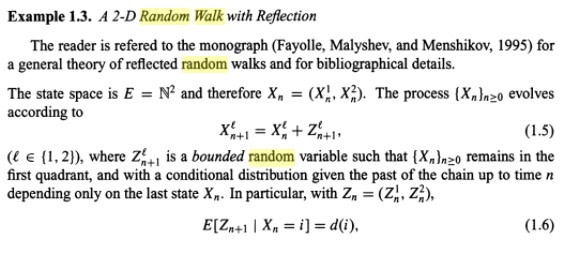
\includegraphics[width=\textwidth]{week12/f_1}
\end{figure}
\begin{figure}[H]
\centering
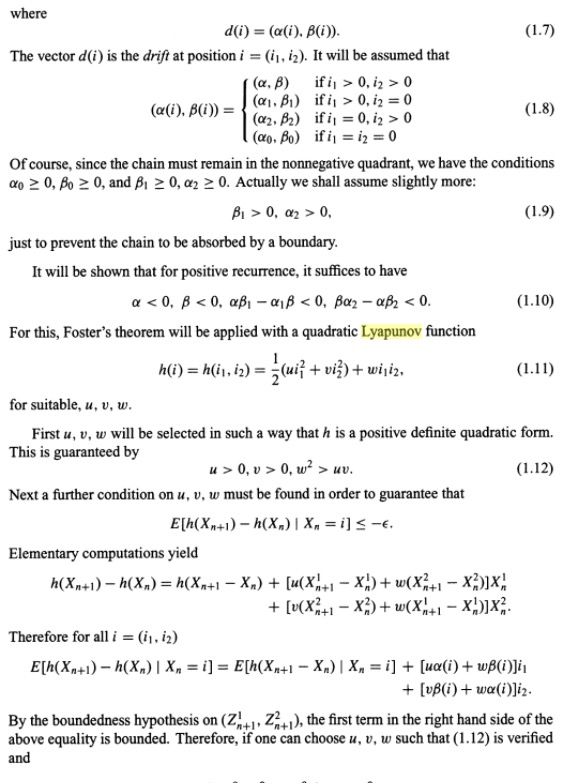
\includegraphics[width=\textwidth]{week12/f_2}
\end{figure}
\begin{figure}[H]
\centering
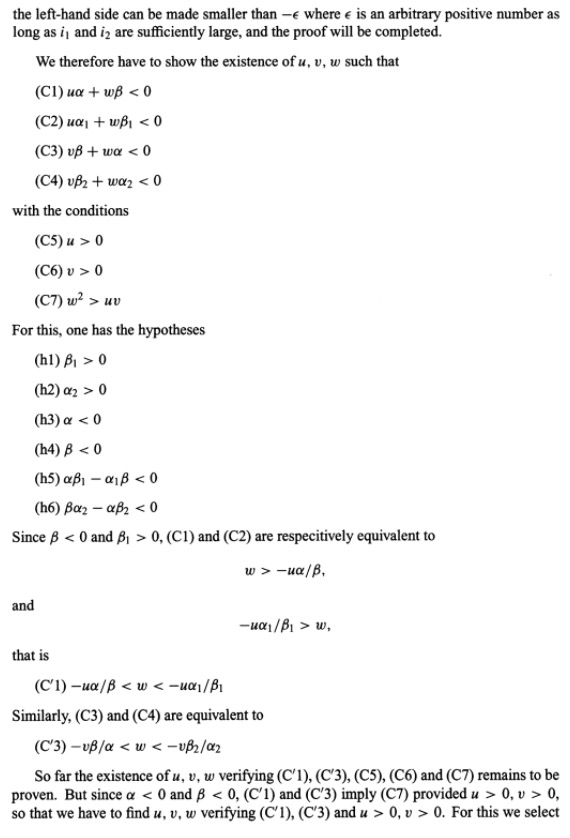
\includegraphics[width=\textwidth]{week12/f_3}
\end{figure}
\begin{figure}[H]
\centering
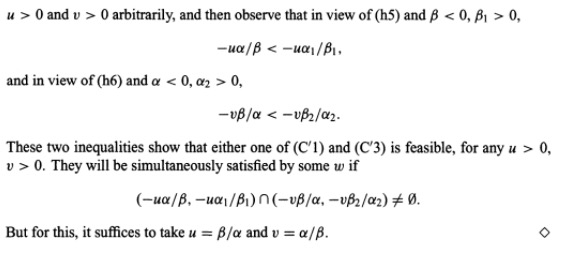
\includegraphics[width=\textwidth]{week12/f_4}
\end{figure}











